\input{../../preamble2.tex}
% \bibliographystyle{plain} % Style BST file (bmc-mathphys, vancouver, spbasic).
% \bibliographystyle{unsrt} % Style BST file (bmc-mathphys, vancouver, spbasic).
\bibliography{pubs.bib}      % Bibliography 

\title{Professional Drone, Hybrid Power Pack  - Timebox 10}
\author{Team 2}

\begin{document}

\lstset{language=Matlab,%
  % basicstyle=\color{red},
    inputencoding=latin1,
    breaklines=true,%
    morekeywords={matlab2tikz},
    keywordstyle=\color{blue},%
    morekeywords=[2]{1}, keywordstyle=[2]{\color{black}},
    identifierstyle=\color{black},%
    stringstyle=\color{mylilas},
    commentstyle=\color{mygreen},%
    showstringspaces=false,%without this there will be a symbol in the places where there is a space
    numbers=left,%
    numberstyle={\tiny \color{black}},% size of the numbers
    numbersep=9pt, % this defines how far the numbers are from the text
    emph=[1]{for,end,break},emphstyle=[1]\color{red}, %some words to emphasise
    %emph=[2]{word1,word2}, emphstyle=[2]{style},    
}


\lstset{language=C,%
  % basicstyle=\color{red},
  inputencoding=latin1,
  breaklines=true,%
  morekeywords={matlab2tikz},
  keywordstyle=\color{blue},%
  morekeywords=[2]{1}, keywordstyle=[2]{\color{black}},
  identifierstyle=\color{black},%
  stringstyle=\color{mylilas},
  commentstyle=\color{mygreen},%
  showstringspaces=false,%without this there will be a symbol in the places where there is a space
  % numbers=left,%
  % numberstyle={\tiny \color{black}},% size of the numbers
  % numbersep=9pt, % this defines how far the numbers are from the text
  emph=[1]{for,end,break},emphstyle=[1]\color{red}, %some words to emphasise
  % emph=[2]{word1,word2}, emphstyle=[2]{style},
}


% \lstdefinestyle{customc}{
%   belowcaptionskip=1\baselineskip,
%   breaklines=true,
%   frame=L,
%   xleftmargin=\parindent,
%   language=C,
%   showstringspaces=false,
%   basicstyle=\footnotesize\ttfamily,
%   keywordstyle=\bfseries\color{green!40!black},
%   commentstyle=\itshape\color{purple!40!black},
%   identifierstyle=\color{blue},
%   stringstyle=\color{orange},
% }

% \lstdefinestyle{customasm}{
%   belowcaptionskip=1\baselineskip,
%   frame=L,
%   xleftmargin=\parindent,
%   language=[x86masm]Assembler,
%   basicstyle=\footnotesize\ttfamily,
%   commentstyle=\itshape\color{purple!40!black},
% }

% \lstset{escapechar=@,style=customc}

\newcounter{udrboks}[section]\setcounter{udrboks}{0}
\renewcommand{\theudrboks}{\arabic{section}.\arabic{udrboks}}
\renewcommand{\theudrboks}{\arabic{udrboks}}
\newenvironment{udrboks}[2][]{%
  \refstepcounter{udrboks}%
  \ifstrempty{#1}%
  {\mdfsetup{%
      frametitle={%
        \tikz[baseline=(current bounding box.east),outer sep=0pt]
        \node[anchor=east,rectangle,fill=blue!20]
        {\strut Udregninger~\theudrboks};}}
  }%
  {\mdfsetup{%
      frametitle={%
        \tikz[baseline=(current bounding box.east),outer sep=0pt]
        \node[anchor=east,rectangle,fill=blue!20]
        {\strut Udregninger ~\theudrboks:~#1};}}%
  }%
  \mdfsetup{innertopmargin=10pt,linecolor=blue!20,%
    linewidth=2pt,topline=true,%
    frametitleaboveskip=\dimexpr-\ht\strutbox\relax
  }
  \begin{mdframed}[]\relax%
    \label{#2}}{\end{mdframed}}


\newcounter{formelboks}[section]\setcounter{formelboks}{0}
\renewcommand{\theformelboks}{\arabic{section}.\arabic{formelboks}}
\renewcommand{\theformelboks}{\arabic{formelboks}}
\newenvironment{formelboks}[2][]{%
  \refstepcounter{formelboks}%
  \ifstrempty{#1}%
  {\mdfsetup{%
      frametitle={%
        \tikz[baseline=(current bounding box.east),outer sep=0pt]
        \node[anchor=east,rectangle,fill=blue!20]
        {\strut Formler~\theformelboks};}}
  }%
  {\mdfsetup{%
      frametitle={%
        \tikz[baseline=(current bounding box.east),outer sep=0pt]
        \node[anchor=east,rectangle,fill=blue!20]
        {\strut Formler ~\theformelboks:~#1};}}%
  }%
  \mdfsetup{innertopmargin=10pt,linecolor=blue!20,%
    linewidth=2pt,topline=true,%
    frametitleaboveskip=\dimexpr-\ht\strutbox\relax
  }
  \begin{mdframed}[]\relax%
    \label{#2}}{\end{mdframed}}

\newcounter{konstboks}[section]\setcounter{konstboks}{0}
\renewcommand{\thekonstboks}{\arabic{section}.\arabic{konstboks}}
\newenvironment{konstboks}[2][]{%
  \refstepcounter{konstboks}%
  \ifstrempty{#1}%
  {\mdfsetup{%
      frametitle={%
        \tikz[baseline=(current bounding box.east),outer sep=0pt]
        \node[anchor=east,rectangle,fill=green!20]
        {\strut Konstanter~\thekonstboks};}}
  }%
  {\mdfsetup{%
      frametitle={%
        \tikz[baseline=(current bounding box.east),outer sep=0pt]
        \node[anchor=east,rectangle,fill=green!20]
        {\strut Konstanter~\thekonstboks:~#1};}}%
  }%
  \mdfsetup{innertopmargin=10pt,linecolor=green!20,%
    linewidth=2pt,topline=true,%
    frametitleaboveskip=\dimexpr-\ht\strutbox\relax
  }
  \begin{mdframed}[]\relax%
    \label{#2}}{\end{mdframed}}
\pgfplotstableread[row sep=\\,col sep=&]{
  ide & stemmer  \\
  Paraply & 9  \\
  Fjernbetjening & 7  \\
  iAdapt & 2 \\
}\mydata
% \setcounter{secnumdepth}{1}
\maketitle
\thispagestyle{empty}

\textbf{Deltagere:}
\begin{figure}[h]
  \centering
  % BEGIN RECEIVE ORGTBL delt
  \begin{tabular}{|p{5cm}p{10cm}|}
    \hline
    &\\
    Stud. nr: 201602094 & Navn: Søren Holm Korsgaard \\
    \hline
    &\\
    Stud.nr.: 201607563 & Navn: Jacob Gustafsson \\
    \hline
    &\\
    % Stud.nr.: 201704859 & Navn: Jonas Buus \\
    % \hline
    % &\\
    Stud.nr.: 20084327 & Navn: Simon Rasmussen \\
    \hline
    &\\
    Stud.nr.: 201704483 & Navn: Thomas Dueholm Jensen \\
    \hline
  \end{tabular}
  % END RECEIVE ORGTBL delt

\end{figure}
\vspace{-5mm}
% \clearpage
\setcounter{tocdepth}{2}
\tableofcontents
\thispagestyle{empty}
\newpage
% \pagenumbering{arabic}
\setcounter{page}{1}

% \section{Introduktion}
% \label{sec:introduktion}

\section{Strategy and planning}
\label{sec:strat-plann-jacob}

I denne timebox præsenteres resultater af test af ensretter samt PID-kontrol. Det er den afsluttende timebox for projekt 4 og der uddybes derfor ikke på videreudvikling.


\section{Aktiv ensretter (Thomas)}
\label{sec:aktiv-ensretter}

I timebox 9 konkluderede vi, at der skulle monteres nye MOSFETS med en lavere intern modstand og/eller påmonteres en heatsink på PCB printet Vi indkøbte derfor følgende MOSFETS

\begin{itemize}
\item $OptiMOS^{TM}5$ Power-transistor
  \begin{itemize}
  \item Max drain strøm: 100 A.
  \item Max drain-source spænding: 100 V.
  \item $R_{DS(on)}$: 3.9 m$\Omega$.
  \item $R_{\theta JA}$: 62 $^\circ$C/W
  \end{itemize}
\end{itemize}

Disse MOSFET transistorer blev monteret på PCB printet, hvorefter samme testprocedure som tidligere blev gennemført.  

Testen resulterede dog i en defekt transistor.

\begin{figure}[h]
  \centering
  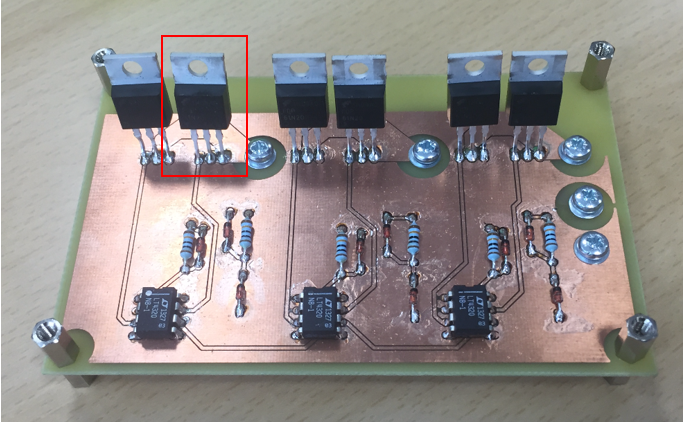
\includegraphics[width=0.7\textwidth]{nt8.png}
  \caption{Defekt transistor. Markeret med rød firkant.}
  \label{fig:nt8}
\end{figure}

Årsagen til defekten var på daværende tidpunkt uafklaret, hvorfor det blev besluttet at måle gate spændingerne på samtlige transistorer i forhold til stel, da vi havde en mistanke om, at der var ubalance i kredsløbet. Ubalance kunne muligvis være årsagen til defekten af den ene transistor. 

Figur \ref{fig:nt9} viser målingen af gate spændingen på de tre transistorer, der håndterer den positive del af inputtet. Hvis kredsløbet fungerede korrekt, skulle der gerne være samme spændingsniveau på samtlige gates. 
\clearpage
\begin{figure}[h]
  \centering
  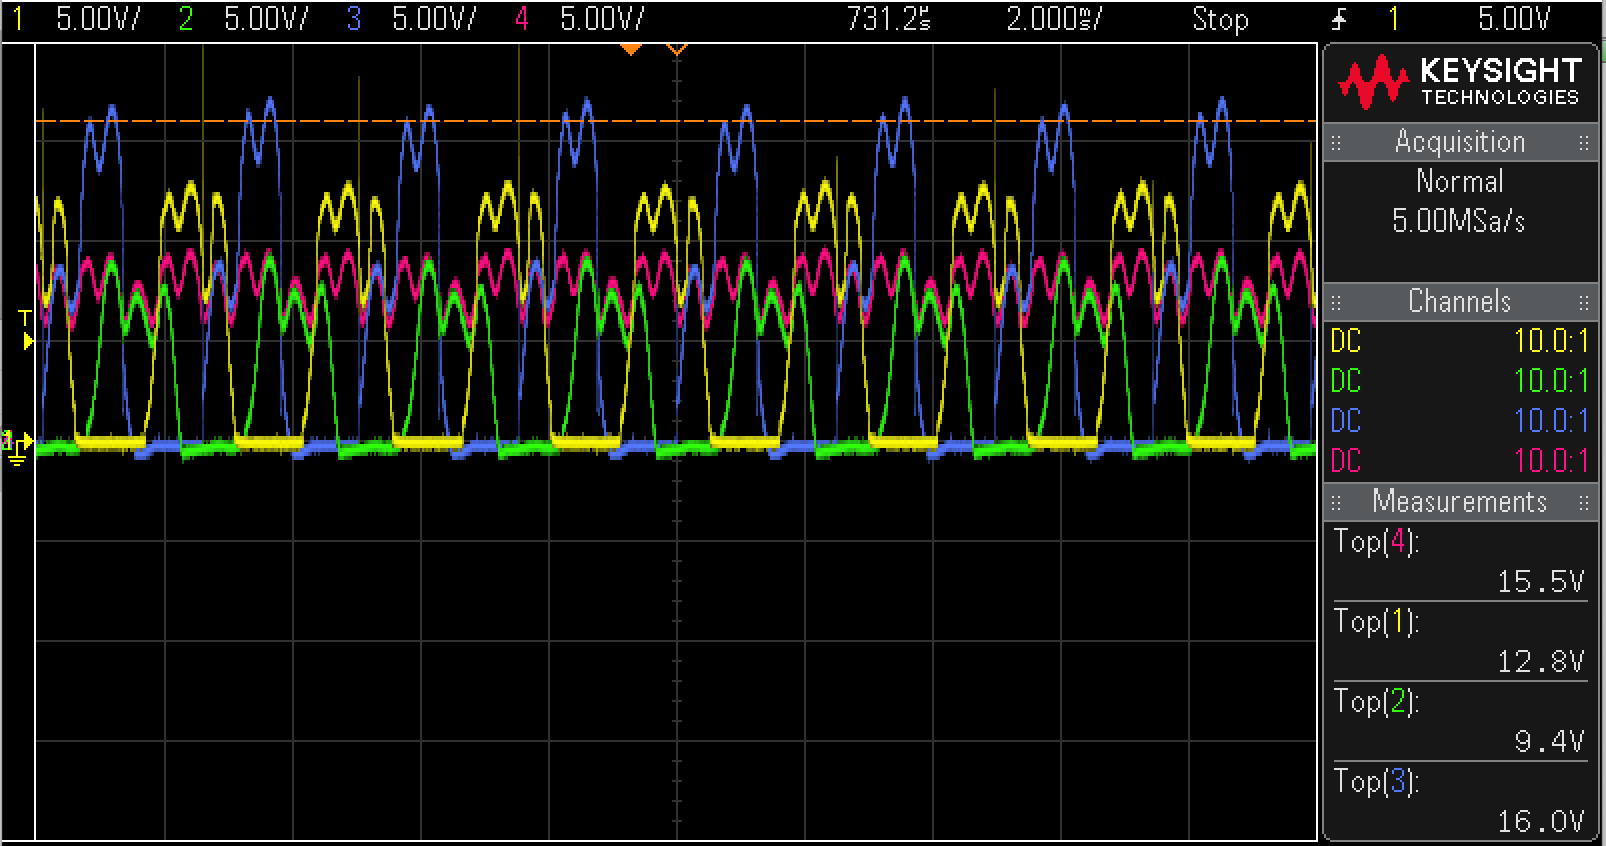
\includegraphics[width=0.7\textwidth]{nt9.png}
  \caption{Gatespænding. Grøn: fase 1+, blå: fase 2+, gul: fase 3+, rød: $V_{out}$}
  \label{fig:nt9}
\end{figure}

Her ses, at gate spændingerne ikke har samme niveau. Peak værdier varierer mellem 9.4 V (fase 1), 12.8 V (fase 2) og 16.0 V (fase 3).

På baggrund af denne måling, og da vi ikke havde mere tid til rådighed, var vi desværre nødsaget til at stoppe udviklingen af den aktive ensretter. 


\section{Motorstyring (Simon)}
\label{sec:motorstyring}

Ved implementering af PID-koden sås desværre insufficient kontrol af omdrejningerne, idet kontrollen fremstod invers, sådan at ved øget omdrejningstal blev gasspjældet mere åbent. Der var afslutningsvis på semesteret desværre ikke tid til mere udvikling.

På baggrund af tidligere PID-kode, se timebox 6 udarbejdes der nu et udkast til PID-kontrol software, som også benytter sig af tidligere udviklet kode til kontrol af servomotor samt aflæsning af motorens omdrejninger.

\lstinputlisting[language=c,basicstyle=\scriptsize\ttfamily]{pidkl25cpp.cpp}  


% \clearpage
% \section{Deployment (Alle)}
% \label{sec:deployment}

% I denne timebox deployes en opnået spændingsregulering fra 22 V til 5,3 V. Herudover deployes udkast til kode der skal aflæse omdrejningstal fra forbrændingsmotoren og desuden deployes de tunede PID-koefficienter.

% Hermed godkender kunderne, Morten Oppbrud Jakobsen og Jan Møller Nielsen, ovenstående i timebox 9.

% Mandag den 13/5-2019

% \begin{minipage}{.5\textwidth}
%   \begin{center}
%     \vspace{1.4cm}
%     \rule{0.8\textwidth}{0.1pt}\\
%     \small{Morten Opprud Jakobsen\\%\vspace{0.1cm}\textit{Projektansvarlig læge}
%     }
%   \end{center}
% \end{minipage}%
% \begin{minipage}{0.5\textwidth}
%   \begin{center}
%     \vspace{1.4cm}
%     \rule{0.8\textwidth}{0.1pt}\\
%     \small{Jan Møller Nielsen\\%\vspace{0.1cm}\textit{Forskningsansvarlig overlæge}
%     }
%   \end{center}
% \end{minipage}

% \printbibliography
\end{document}